\documentclass[table]{beamer}

\usepackage{kotex}
\usepackage{amsmath}
\usepackage{amssymb}
\usepackage{verbatim}
\ifxetex
 \setsansfont{TeX Gyre Heros}
 \setsanshangulfont{맑은 고딕}
\fi
\usepackage{color, colortbl}					%tabular에서 rowcolor를 변경하기 위해서..
\usepackage{fancybox}
\usepackage{graphbox,graphicx}
\usepackage{tikz}								%오버레이에 그림을 그리기 위해서..
\usepackage{hyperref}							%하이퍼링크 처리

\usepackage{array}
\usepackage{ebproof}
\usepackage{multirow}


\usepackage{xcolor,multirow}
\usepackage{hhline}

\usepackage[T1]{fontenc}
\usepackage{textcomp}
\usepackage{listings}							%자바 코드를 위해서..
\lstset{
	mathescape,
	language=Java,
	basicstyle=\footnotesize\ttfamily,
	keywordstyle={}, % \footnotesize\color{blue}\ttfamily,
	captionpos=b,
	escapeinside=@@,
	showstringspaces=false,					%공백 문제 제거를 위해서
	tabsize=2,
	upquote=true
}

%----------------- 총 페이지수에서 백업 슬라이드를 제거하기 위해서....
\newcommand{\backupbegin}{
   \newcounter{framenumberappendix}
   \setcounter{framenumberappendix}{\value{framenumber}}
}
\newcommand{\backupend}{
   \addtocounter{framenumberappendix}{-\value{framenumber}}
   \addtocounter{framenumber}{\value{framenumberappendix}} 
}
%-----------------

%---------------- tabular에서 rowcolor를 변경하기 위해서..
\definecolor{Gray}{gray}{0.9}
%-----------------

%\usetheme{CambridgeUS}
% \usecolortheme{default}

\usetheme{default}
\usecolortheme{default}

%\usetheme{default}
%\usecolortheme{beaver}
%\usetheme{CambridgeUS}
%\usecolortheme{seagull}

%\useinnertheme{rectangles}


\setbeamertemplate{caption}{\insertcaption}	%그림의 캡션 자동 만들지 않도록.

\addtobeamertemplate{navigation symbols}{}{%
    \usebeamerfont{footline}%
    \usebeamercolor[fg]{footline}%
    \hspace{1em}%
    \insertframenumber/\inserttotalframenumber
}

\title[Types and Programming Languages]{9. Simply Typed Lambda-Calculus \\
(Types and Programming Languages)}
\author[K. Choi]{Kwanghoon Choi}
\institute[Chonnam National University]{
Software Languages and Systems Laboratory \\
	Chonnam National University}
\date{Week 6}

%%%%% Macros %%%%%

\newcommand{\rpc}{$\lambda_{rpc}$}
\newcommand{\polyrpc}{$\lambda_{rpc}^{\forall}$}
\newcommand{\stateencrpc}{$\lambda_{rpc}^{enc}$}
\newcommand{\statefulrpc}{$\lambda_{rpc}^{state}$}

\newcommand{\cs}{$\lambda_{cs}$}
\newcommand{\stateenccs}{$\lambda_{cs}^{enc}$}
\newcommand{\statefulcs}{$\lambda_{cs}^{state}$}

\newcommand{\client}{\textbf{c}}
\newcommand{\server}{\textbf{s}}
\newcommand{\clientserver}{\textbf{cs}}

\newcommand{\Loc}{Loc}

\newcommand{\evalRPC}[3]{#1\Downarrow_{#2}#3}
\newcommand{\evalRPCC}[2]{#1\Downarrow_{\client}#2}
\newcommand{\evalRPCS}[2]{#1\Downarrow_{\server}#2}
\newcommand{\lamL}[3]{\lambda^{#1}#2.#3}
\newcommand{\appL}[3]{#1{\ }^{#2}#3} 
\newcommand{\subst}[2]{\{#1/#2\}}
\newcommand{\llet}[3]{\textsf{let} \ #1 = #2 \ \textsf{in} \ #3}

\newcommand{\textsfReq}{\textsf{req}}
\newcommand{\req}[2]{\textsfReq(#1,#2)}
\newcommand{\reqwith}[3]{\textsfReq_{#1}(#2,#3)}

\newcommand{\textsfCall}{\textsf{call}}
\newcommand{\call}[2]{\textsfCall(#1,#2)}
\newcommand{\callwith}[3]{\textsfCall_{#1}(#2,#3)}

\newcommand{\textsfRet}{\textsf{ret}}
\newcommand{\ret}[1]{\textsfRet(#1)}
\newcommand{\retwith}[2]{\textsfRet_{#1}(#2)}

\newcommand{\funL}[1]{\xrightarrow{#1}}    
\newcommand{\funLC}[2]{\xrightarrow[#2]{#1}}  
\newcommand{\tyenv}{\Gamma}     
\newcommand{\tyenvExt}[2]{\Gamma\{#1:#2\}}
\newcommand{\tyenvExtWith}[1]{\Gamma,#1}
% \newcommand{\typing}[4]{#1\rhd_{#2} #3 : #4}       
\newcommand{\typing}[4]{#1\vdash_{#2} #3 : #4}       
\newcommand{\typingBlack}[4]{#1\blacktriangleright_{#2} #3 : #4}  

\newcommand{\loceta}[2]{{#1}\rightsquigarrow{#2}}                                         

\newcommand{\enc}{\textsf{enc}}
\newcommand{\evalStateEncRPCC}[2]{$#1\Downarrow_{\client}^{\enc}#2$}
\newcommand{\evalStateEncRPCS}[3]{$#1;#2\Downarrow_{\server}^{\enc}#3$}

\newcommand{\sta}{\textsf{state}}
\newcommand{\evalStatefulRPCC}[3]{\evalStatefulRPC{#1}{#2}{\client}{#3}}
\newcommand{\evalStatefulRPCS}[3]{\evalStatefulRPC{#1}{#2}{\server}{#3}}
\newcommand{\evalStatefulRPC}[4]{${#1};{#2}\Downarrow_{#3}^{\sta}{#4}$}

\newcommand{\deep}{\textsf{deep}}
\newcommand{\evalDeeplyStatefulRPCC}[3]{\evalDeeplyStatefulRPC{#1}{#2}{\client}{#3}}
\newcommand{\evalDeeplyStatefulRPCS}[3]{\evalDeeplyStatefulRPC{#1}{#2}{\server}{#3}}
\newcommand{\evalDeeplyStatefulRPC}[4]{${#1};{#2}\Downarrow_{#3}^{\deep}{#4}$}

\newcommand{\IdK}{\textsf{Id}}
\newcommand{\FunK}[3]{\textsf{Fun} \ #2 \ #3}
\newcommand{\AppK}[3]{\textsf{App} \ #2 \ #3}
%\newcommand{\FunK}[3]{\textsf{Fun}^{#1} \ #2 \ #3}
%\newcommand{\AppK}[3]{\textsf{App}^{#1} \ #2 \ #3}
                                                
\newcommand{\reify}[1]{\ulcorner #1 \urcorner}

\newcommand{\RightarrowEnc}{\Rightarrow^{enc}}
\newcommand{\RightarrowEncStar}{\Rightarrow^{enc*}}
\newcommand{\RightarrowEncPlus}{\Rightarrow^{enc+}}

\newcommand{\runStateEncRPC}[2]{$#1 \RightarrowEnc #2$}
\newcommand{\runStateEncRPCStar}[2]{$#1 \RightarrowEncStar #2$}
\newcommand{\runStateEncRPCPlus}[2]{$#1 \RightarrowEncPlus #2$}

\newcommand{\runStateEncCS}[2]{$#1 \Rightarrow^{enc} #2$}
\newcommand{\runStateEncCSStar}[2]{$#1 \Rightarrow^{enc*} #2$}

\newcommand{\runStatefulRPC}[2]{$#1 \Rightarrow^{state} #2$}
\newcommand{\runStatefulRPCStar}[2]{$#1 \Rightarrow^{state*} #2$}

\newcommand{\runStatefulCS}[2]{$#1 \Rightarrow^{state} #2$}
\newcommand{\runStatefulCSStar}[2]{$#1 \Rightarrow^{state*} #2$}

\newcommand{\emp}{\epsilon}
\newcommand{\substzsxs}{\{\bar{v}/\bar{z},\overline{w}/\bar{x} \}}
\newcommand{\substxs}{\{\overline{w}/\bar{x} \}}

\newcommand{\substZsXs}{\{\overline{V}/\bar{z},\overline{W}/\bar{x} \}}
\newcommand{\substXs}{\{\overline{W}/\bar{x} \}}

\newcommand{\LetK}[2]{\textsf{ctx}\ #1 \ #2}
%\newcommand{\LetK}[2]{(#1,#2)}
\newcommand{\opt}[1]{#1_{opt}}

\newcommand{\overlineK}{\overline{K}}
\newcommand{\overlinePi}{\overline{\Pi}}
\newcommand{\overlineDelta}{\overline{\Delta}}

%\newcommand{\comp}[1]{\rightsquigarrow_{#1}}
%\newcommand{\comps}{\rightsquigarrow_{\server}}
%\newcommand{\compc}{\rightsquigarrow_{\client}}
\newcommand{\ccomp}[1]{C[\![#1]\!]}
\newcommand{\scomp}[1]{S[\![#1]\!]}
\newcommand{\vcomp}[1]{V[\![#1]\!]}
\newcommand{\cconv}[1]{CC[\![#1]\!]}
%\newcommand{\cconvprg}[1]{CC_{prg}[\![#1]\!]}

\newcommand{\FUNS}{\Phi}
\newcommand{\fv}[1]{\textsf{fv}(#1)}
\newcommand{\dom}[1]{\textsf{dom}(#1)}
\newcommand{\clo}[2]{clo({#1},{#2})}

\newcommand{\sessionNothing}{\makebox[0.3cm][c]{\scriptsize $nothing$}}
\newcommand{\sessionSomething}{\makebox[0.3cm][c]{\scriptsize $session$}}
\newcommand{\sessionOption}{\makebox[0.3cm][c]{\scriptsize $optSession$}}

\newcommand{\mono}[1]{[\![#1]\!]}

\newcommand{\eqdef}{\overset{\mathrm{def}}{=\joinrel=}}

%%
%\newtheorem{lemma}{Lemma}[section]
%\newtheorem{theorem}{Theorem}[section]
%\newtheorem{fact}{Fact}[section]
%\newtheorem{definition}{Definition}[section]

%%%%%%%%%%%%%%%%%%

\begin{document}

%\section{Relative Pronoun}
\begin{frame}
%\begin{center}
%{\footnotesize
%Types and Programming Languages
%}
%\end{center}
	\titlepage
	
%	\begin{center}
%	{
%  (Joint work with James Cheney, Simon Fowler, and Sam Lindley)
%	}
%	\end{center}
\end{frame}

%\begin{frame}{Table of Contents}
%\begin{itemize}
%\item
%\item
%\item
%\item
%\end{itemize}
%\end{frame}

%%%
\begin{frame}[t]{Overview} \vspace{10pt}

This chapter introduces the most elementary member of the family of typed languages: the simply typed lambda-calculus of Church (1940) and Curry (1958).

\end{frame}

%%%
\begin{frame}[t]{9.1 Function Types} \vspace{10pt}

Recall that in the type system for the arithmetic PL with two types:
\begin{itemize}
\item Bool: classifying terms whose evaluation yields a boolean
\item Nat: classifying terms whose evaluation yields a number
\end{itemize}

\vspace{10pt}

The ``ill-typed'' terms not belonging to either of these types include all the terms that reach stuck states during evaluation
\begin{itemize}
\item e.g., if 0 then 1 else 2
\end{itemize}
as well as some terms that actually behave fine during evaluation but for which our static classification is too conservative
\begin{itemize}
\item e.g., if true then 0 else false.
\end{itemize}

\vspace{10pt}

To extend the type system to include functions, we need to add a type classifying terms whose evaluation results in a function.

\end{frame}

%%%
\begin{frame}[t]{9.1 Function Types (Cont.)} \vspace{10pt}

To extend the type system to include functions, we need to add a type classifying terms whose evaluation results in a function.

\vspace{10pt}

The first trial: to add a typing rule ``$\lambda$x.t : $\rightarrow$'' giving every lambda-abstraction the type $\rightarrow$. 
\begin{itemize}
\item Good to classify lambda-abstractions from booleans and numbers, but

\item Too conservative: functions like $\lambda$x.true and $\lambda$x.$\lambda$y.y are in the same type $\rightarrow$, 

%\item ignoring the fact that applying the first to {\texttt true} yields a boolean while applying the second to {\texttt true} yields another function.
\end{itemize}

\vspace{10pt}

We need to know what type the function returns and what type of arguments it expects: T1 $\rightarrow$ T2

\end{frame}

%%%
\begin{frame}[t]{9.1 Function Types (Cont.)} \vspace{10pt}

The syntax of types in the lambda calculus
\[
T \ ::= \ Nat \ \ \ | \ \ \ Bool \ \ \ | \ \ \ T \rightarrow T 
\]

\vspace{10pt}

\begin{itemize}
\item
Bool $\rightarrow$ Bool is the type of functions mapping boolean arguments to boolean results.

\item
``T1 $\rightarrow$ T2 $\rightarrow$ T3'' denotes T1 $\rightarrow$ (T2 $\rightarrow$ T3), \\ not (T1 $\rightarrow$ T2) $\rightarrow$ T3.


\item
(Bool $\rightarrow$ Bool) $\rightarrow$ (Bool $\rightarrow$ Bool)--or, equivalently, (Bool $\rightarrow$ Bool) $\rightarrow$ Bool $\rightarrow$ Bool

\begin{itemize}
\item[:] the type of functions that take boolean-to-boolean functions as arguments and return them as results.
\end{itemize}
\end{itemize}

\end{frame}

%%%
\begin{frame}[t]{9.2 The Typing Relation} \vspace{10pt}

In order to assign a type to an abstraction $\lambda$x.t, we need to know what type of arugments to expect. 

\vspace{10pt}

The explicitly typed approach with $\lambda$x:T. t annotates the type to the argument of the abstraction. 

\vspace{10pt}

The other approach infers the type (T) of the argument (x) based on how the argument is used in the body of the abstraction (t).

\vspace{10pt}

The type of the function's result is the type of the body t2, where occurrences of x in t2 are assumed to denote terms of type T1:
\begin{center}
\begin{prooftree}
\hypo{ \texttt{x:T1 $\vdash$ t2 : T2 } }
\infer1[]{ \texttt{$\vdash$ $\lambda$x:T1.t2 : T1$\rightarrow$T2 }}
\end{prooftree}
\end{center}

\vspace{10pt}

``$\Gamma$ $\vdash$ t : T'' instead of ``t : T'' where $\Gamma$ = \{ x1:T1, ... , xk:Tk \}.

\end{frame}

%%%
\begin{frame}[t]{9.2 The Typing Relation (Cont.)} \vspace{10pt}

Pure simply typed lambda-calculus ($\lambda_{\rightarrow}$)

\vspace{10pt}

\begin{tabular}{l l c l}
Types & T & ::= & Nat \ \ \ | \ \ \ Bool \ \ \ | \ \ \ T $\rightarrow$ T \\
Terms & t & ::= & x \ \ \ | \ \ \ $\lambda$ x:T.t \ \ \ | \ \ \ t \ t \\
Values & v & ::= & $\lambda$ x:T.t 
\end{tabular}

\vspace{10pt}

Typing rules

\vspace{10pt}

\begin{tabular}{c c}
\mbox{
\begin{prooftree}
\hypo{ \texttt{$\Gamma$(x)=T} }
\infer1[]{ \texttt{$\Gamma$ $\vdash$ x : T} }
\end{prooftree}
}
&
(T-Var)\\[0.5cm]
\mbox{
\begin{prooftree}
\hypo{ \texttt{$\Gamma$, x:T1 $\vdash$ t : T2} }
\infer1[]{ \texttt{$\Gamma$ $\vdash$ $\lambda$x.t : T1 $\rightarrow$ T2} }
\end{prooftree}
}
&
(T-Abs)\\[0.5cm]
\mbox{
\begin{prooftree}
\hypo{ \texttt{$\Gamma$ $\vdash$ t1 : T1 $\rightarrow$ T2} }
\hypo{ \texttt{$\Gamma$ $\vdash$ t2 : T1} }
\infer2[]{ \texttt{$\Gamma$ $\vdash$ t1 t2 : T2} }
\end{prooftree}
}
&
(T-App)\\[0.5cm]
\end{tabular}
\end{frame}

%%%
\begin{frame}[t]{9.2 The Typing Relation (Cont.)} \vspace{10pt}

Typing rules for the boolean constants and conditional expressions are the same as before.

\vspace{10pt}

\begin{tabular}{c c}
\mbox{
\begin{prooftree}
\hypo{ \texttt{$\Gamma$ $\vdash$ t1 : Bool} }
\hypo{ \texttt{$\Gamma$ $\vdash$ t2 : T} }
\hypo{ \texttt{$\Gamma$ $\vdash$ t3 : T} }
\infer3[]{ \texttt{$\Gamma$ $\vdash$ if t1 then t2 else t3 : T} }
\end{prooftree}
}
&
(T-If)\\[0.5cm]
\end{tabular}

\vspace{10pt}

cf.

\vspace{10pt}

\begin{tabular}{c c}
\mbox{
\begin{prooftree}
\hypo{ \texttt{t1 : Bool} }
\hypo{ \texttt{t2 : T} }
\hypo{ \texttt{t3 : T} }
\infer3[]{ \texttt{ if t1 then t2 else t3 : T} }
\end{prooftree}
}
&
\\[0.5cm]
\end{tabular}

\vspace{10pt}

Q. Rewrite all the typing rules for the arithmetic PL in 3-ary relation. 

\end{frame}

%%%
\begin{frame}[t]{9.2 The Typing Relation (Cont.)} \vspace{10pt}

The typing derivation for ``($\lambda$x:Bool. x) true''

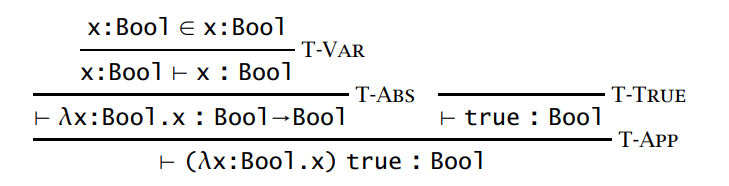
\includegraphics[width=10cm]{typingderivation_ch9}

\vspace{10pt}

Note that we write $\vdash$ t : T  (or $\emptyset \vdash$ t : T)  when $\Gamma$ is empty.

\vspace{10pt}

Q. Show (by drawing derivation trees) that the following terms have the indicated types:

\begin{itemize}
\item f:Bool$\rightarrow$Bool $\vdash$ f (if false then true else false) : Bool
\item f:Bool$\rightarrow$Bool $\vdash$ $\lambda$x:Bool. f (if x then false else x) : Bool$\rightarrow$Bool
\end{itemize}

\end{frame}

%%%
\begin{frame}[t]{9.2 The Typing Relation (Cont.)} \vspace{10pt}

Q Find a context $\Gamma$ under which the term ``f x y'' has type Bool. 

\vspace{10pt}

Q. Can you give a simple description of the set of {\it all} such contexts?

\end{frame}

%%%
\begin{frame}[t]{9.3 Properties of Typing} \vspace{10pt}

The property of the type system for the lambda calculus is safety (also called soundness)

\begin{itemize}
\item If \texttt{$\vdash$ t : T}, then the evaluation of the term, \texttt{t}, will never get stuck. 
\item cf. The stuck terms in the lambda calculus are not values but have no progress by the evaluation rules.
\end{itemize}

\vspace*{10pt}

We show the type safety by proving two properites: (1) progress and (2) preservation


\end{frame}

%%%
\begin{frame}[t]{9.3 Properties of Typing (Cont.)} \vspace{10pt}

Progress: A well-typed term is not stuck (either it is a value or it can take a step according to the evaluation rules).

\vspace{10pt}

Theorem[Progress] Suppose t is a closed term. If \texttt{$\vdash$ t : T} then 
\begin{itemize}
\item either \texttt{t} is a value 
\item or there is some \texttt{t'} with $\texttt{t}\rightarrow\texttt{t'}$.
\end{itemize}

\vspace{10pt}

Q. Prove this theorem by induction on typing derivations \texttt{$\vdash$ t : T}.

\end{frame}

%%%
\begin{frame}[t]{9.3 Properties of Typing (Cont.)} \vspace{10pt}

Preservation: If a well-typed term takes a step of evaluation, then the resulting term is also well-typed.

\vspace{10pt}

Theorem[Preservation] 
If \texttt{$\Gamma\vdash$ t : T} and $\texttt{t}\rightarrow\texttt{t'}$ then \texttt{$\Gamma\vdash$ t' : T}.

\vspace{10pt}

Q. Prove this theorem by induction on a derivation of \texttt{$\Gamma\vdash$ t : T} using the following substitution lemma.

\vspace{30pt}

Lemma[Preservation of types under substitution] If \texttt{$\Gamma$,x:S $\vdash$ t:T} and \texttt{$\Gamma\vdash$s:S}, then \texttt{$\Gamma\vdash$ [x$\mapsto$s]t:T}.
\begin{itemize}
\item Provable by induction on a derivation of the statement \texttt{$\Gamma$,x:S$\vdash$t:T}. 
\end{itemize}

\end{frame}

%%%
\begin{frame}[t]{9.4 The Curry-Howard Correspondence} \vspace{10pt}

A connection between type theory and logic known as the {\it Curry-Howard correspondence} or {\it Curry-Howard isomorphism} (Curry and Feys, 1958; Howard, 1980).

\vspace{10pt}

The idea is that, in constructive logics, a proof of a porposition $p$ consists of concrete {\it evidence} for $P$. 

\vspace{10pt}

For example,
\begin{itemize}
\item A proof of a proposition $P \supset Q$ can be viewed as a mechanical procedure that, given a proof of $P$, constructs a proof of $Q$.
\item A proof of $P \wedge Q$ consists of a proof of $P$ together with a proof of $Q$. 
\end{itemize}

\end{frame}

%%%
\begin{frame}[t]{9.4 The Curry-Howard Correspondence (Cont.)} \vspace{10pt}

This observation gives rise to the following correspondence:

 \vspace{10pt}

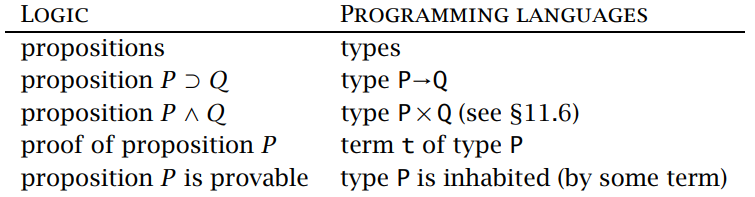
\includegraphics[width=10cm]{curryhowardisomorphism_ch9}

 \vspace{10pt}

On this view, a term of the simply typed lambda calculus is a proof of a logical proposition corresponding to its type. 

\vspace{10pt}

Computation-reduction of lambda-terms- corresponds to the logical operation of proof simplification by {\it cut elimination}. 

\end{frame}

%%%
\begin{frame}[t]{9.4 The Curry-Howard Correspondence (Cont.)} \vspace{10pt}

The beauty of the Curry-Howard correspondence is that it can be extended to a huge variety of type systems and logics. 

%\vspace{10pt}

%\begin{tabular}{l l} \hline
%Type system & Logic \\ \hline
%System F & Second-order constructive logic \\
%System F$_\omega$ & A higher-order logic \\
%Linear type systems & Linear logic \\
%Partial evaluation & Modal logic \\
%Session types (Concurrency) & Linear logic \\ \hline
%\end{tabular}

\begin{center}
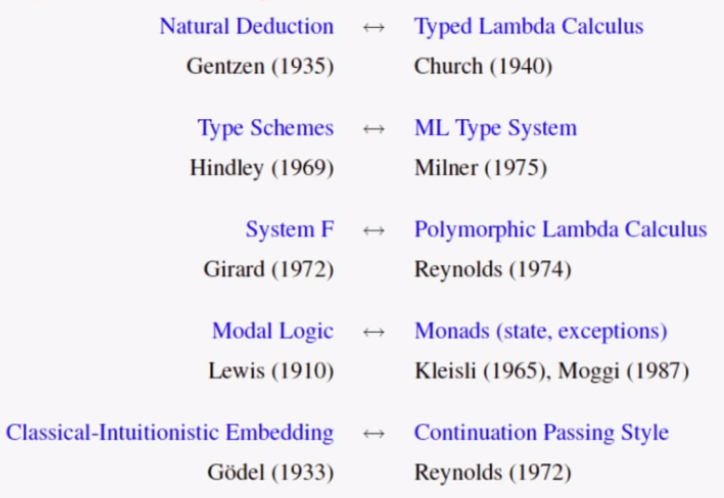
\includegraphics[width=9cm]{curryhowardcorrespondence_wadler_ch9}
\end{center}

\end{frame}

%%%
\begin{frame}[t]{9.5 Erasure and Typability} \vspace{10pt}

We have defined the evaluation relation directly on simply typed terms. But programs can be converted back to an untyped form before they are evaluated. 

\vspace{10pt}

\end{frame}

%%%
\begin{frame}[t]{9.6 Curry-style vs. Church-style} \vspace{10pt}

{\it Curry-style} : Semantics is prior to typing.

\vspace{10pt}

{\it Church-style} : Typing is prior to semantics.

\vspace{10pt}

Implicitly typed presentations of lambda-calculi are often given in the Curry style, while Church-style presentations are common only for explicitly typed systems. 

\end{frame}

\end{document}

